%% Figure 1: one orphan as photo, hand copy and digital transliteration (KBo 24.8, CTH 470).
%% Images: paper/figures/fetch_fragment_images.sh (not in git). Transliteration: TLHdig 0.4, KBo 24.8.
\newcommand{\hb}[1]{{\fontspec{Noto Sans Display}#1}}   % half brackets, missing in Termes
\newcommand{\hit}[1]{\textit{#1}}                         % Hittite and Akkadograms in italics
\begin{figure*}[!t]
  \centering
  \begin{minipage}[c]{0.26\linewidth}\centering
    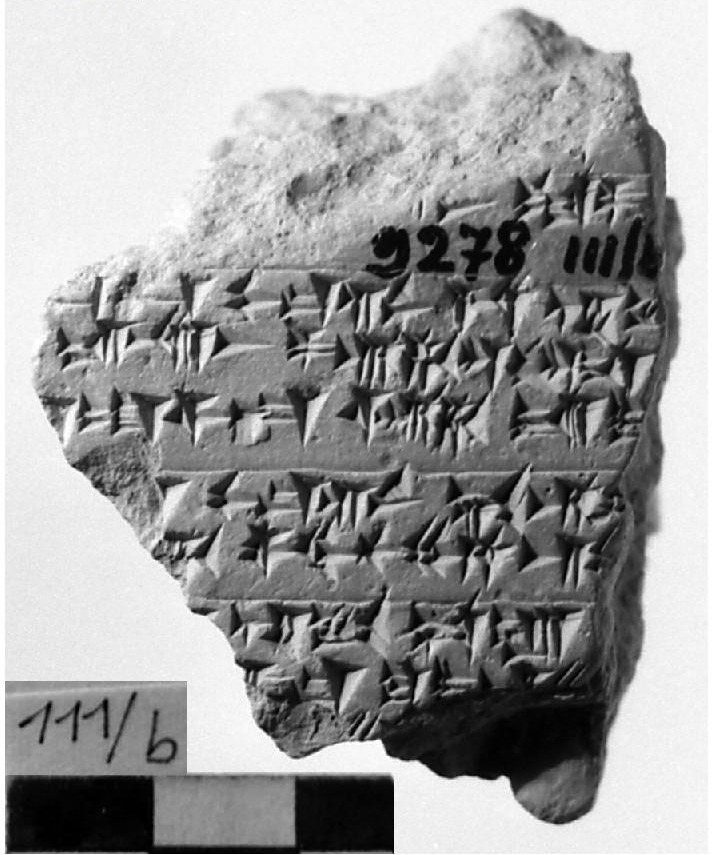
\includegraphics[height=5.2cm]{external/KBo_24_8_photo.jpg}\\[2pt]
    {\footnotesize (a) Photograph}
  \end{minipage}\hfill
  \begin{minipage}[c]{0.30\linewidth}\centering
    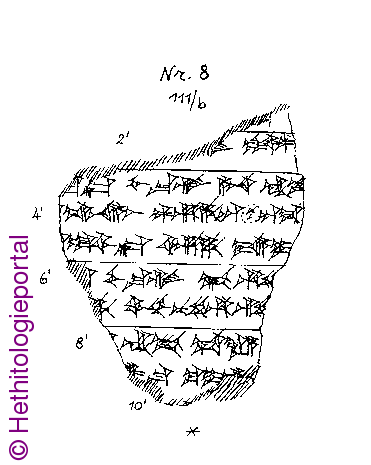
\includegraphics[height=5.2cm]{external/KBo_24_8_handcopy.png}\\[2pt]
    {\footnotesize (b) Hand copy}
  \end{minipage}\hfill
  \begin{minipage}[c]{0.40\linewidth}
    \small
    \begin{tabular}{@{}r@{\hspace{6pt}}l@{}}
      1$'$  & ]x \\
      2$'$  & \{MUNUS\}ŠU.G]I EGIR-\hit{pa} [ \\
      3$'$  & ]x-\hit{kán} \{MUNUS\}ŠU.GI \hit{A-NA} EN SIS[KUR \\
      4$'$  & ]x \hit{iš-na-a-aš pa-tal-ḫa-an} (erasure) \hit{an-da} [ \\
      5$'$  & ]x-\hit{at-ši-kán ar-ḫa da-a-i} [ \\
      6$'$  & ]x \{MUNUS\}ŠU.GI \{DUG\}\hit{ḫu-p}[\hit{u-} \\
      7$'$  & \hit{ar-ḫ}]\hit{a wa-aḫ-nu-uz-zi} [ \\
      8$'$  & ]x EN SISKUR \hit{ša-ra-a} [ \\
      9$'$  & U]DU-\hit{ŠU ku-i-}\hb{⸢}\hit{e}\hb{⸣}\hit{-e}[\hit{š} \\
      10$'$ & ]x x[ \\
    \end{tabular}\\[4pt]
    {\footnotesize (c) Digital transliteration (TLHdig)}
  \end{minipage}
  \caption{An orphan: KBo 24.8, filed under \CTH{470} ``fragments of rituals''. (a) Photograph
    (hethiter.net/: fotarch N08917). (b) Hand copy (KBo 24, no.~8; Hethitologie-Portal Mainz).
    (c) Its transliteration in TLHdig 0.4. The Old Woman (MUNUS ŠU.GI) and the ritual patron (EN
    SISKUR) are visible on the tablet; the method places the fragment with the Luwian rituals of
    Puriyanni and Kuwattalla.}
  \label{fig:fragment}
\end{figure*}
